\section{Integraltransformation}
	\subsection{Allgemein zu transformierbaren Funktionen}
	Ist eine Funktion $f:D\to \C$ gegeben, so erhalten wir die transformierte Funktion $\mathcal{A}f$ durch ein Parameterintegral
	\begin{equation}
		\mathcal{A}f(s) = \int_D k(t,s) f(t) dt \qquad \text{für } s \in G
	\end{equation}
	Die neue Funktion ist somit durch $f$ und den Ausdruck $k: G\times D \to \C$ festgelegt. $k$ ist dabei der Kern des Integraloperators $\mathcal{A}$. \newline
	Eine Integraltransformation ist somit durch ihre Definitionsmenge und ihren Kern definiert.
	\begin{bsp}
		Laplace: \newline
		\begin{equation}
			f(t) = 1 \Rightarrow \mathcal{L}f(t) = \int_0^\infty 1 \cdot e^{-st} dt = -\frac{1}{s} e^{-st}\Big |_0^\infty = \frac{1}{s}
		\end{equation}
	\end{bsp}
	\begin{bem}
		Man spricht bei Abbildungen die Funktionen auf Funktionen abbilden von Operatoren.
	\end{bem}
	\begin{bem} $\;$ \newline
		\begin{itemize}
		\vspace{-0.5cm}
			\item $\mathcal{A}$ ist ein linearer Operator, d.h. es gilt
			\begin{equation}
				\mathcal{A}(\alpha f + \beta g) = \alpha \mathcal{A} f + \beta \mathcal{A} g
			\end{equation}
			\item Es existiert eine Inverse $\mathcal{A}^{-1}$ zu $\mathcal{A}$
		\end{itemize}
	\end{bem}
	
	\subsubsection{Schema bei Integraltransformationen}
	  \begin{figure}[H] 
		  \centering
		  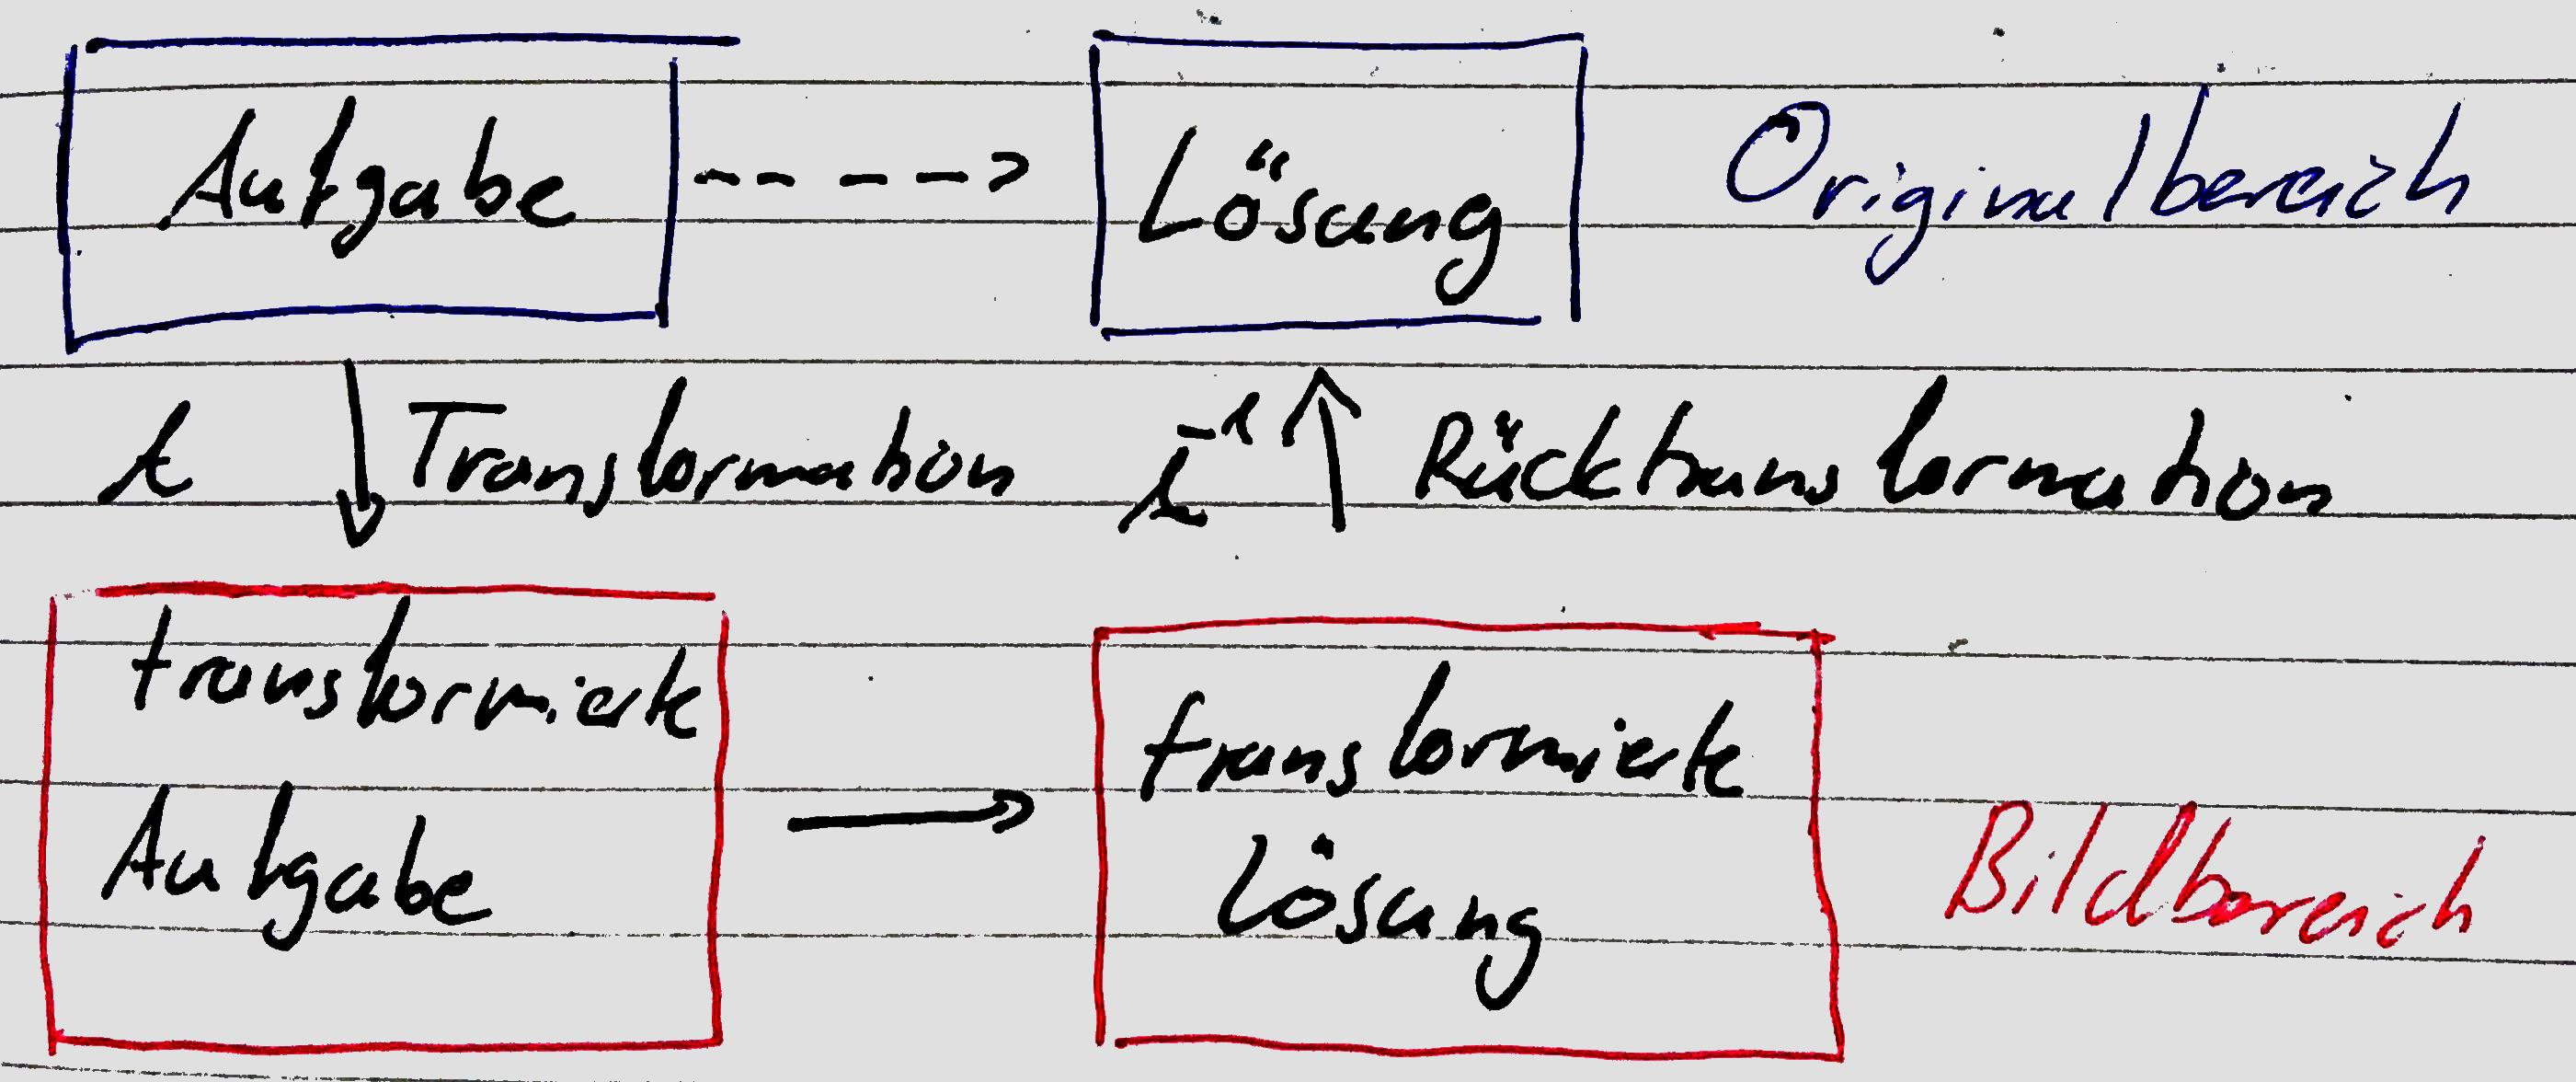
\includegraphics[width=0.5\textwidth]{./img/lapl_trans_allg_a}
		  \caption{Schema Transformation}
		  \label{fig:lapl_trans_allg_schema}
	  \end{figure}
	  
	  Oft lassen sich DGL im Bildbereich einfacher lösen als im Originalbereich. 
	  \begin{bem}
	  	Schreibweise: 
	  	\begin{align*}
	  		\begin{array}{c c c}
	  		\text{Originalbereich} & \; & \text{Bildbereich} \\
	  		f & \laplace & \mathcal{L} \\
	  		1 & \laplace & \frac{1}{s}
	  		\end{array}
	  	\end{align*}
	  \end{bem}
	  
	\subsection{Laplace Transformation}
	\begin{satz}
		Zu einer Funktion $f:[0,\infty) \to \C$ ist auf einem Intervall $J \leq \R \geq 0$ die Laplacetransformierte definiert als die Funktion $\mathcal{L}f:J\to \C$ durch das Parameterintegral
		\begin{equation}
			\mathcal{L}f(s) = \int_0^\infty f(t) e^{-st}dt \qquad,s \in J
		\end{equation}
		gegeben ist, wenn das Integral für $s \in J$ exstiert.
	\end{satz}	
	\begin{bsp}
		\begin{align*}
			f(t) &= \begin{cases}
				1 \qquad, 0 \leq t \leq 1 \\
				0 \qquad, t > 1
			\end{cases}  \\
			\Rightarrow \mathcal{L}f(s) &= \int_0^1 e^{st} \;dt = -\frac{1}{s} e^{-st} \Big |_0^1 = -\frac{1}{s}e^{-s}+\frac{1}{s} = \frac{1}{s}(1-e^{-s})
		\end{align*}
	\end{bsp}
	Hierzu seien folgende wichtigen Laplacetransformierte genannt (aus VL, also in Prüfung nutzbar):
	\renewcommand{\arraystretch}{1.8}
	\begin{align}
		\begin{array}{c | c | l}
		f(t) & F(s) & \text{Anmerkungen}\\ \hline 
		1 &\displaystyle\frac{1}{s} & s > 0 \\
		t^n &  \displaystyle\frac{n!}{s^{n+1}} & s> 0 \\
		e^{kt} &  \displaystyle\frac{1}{s-k} & s > k \in \R \\
		\cos (\omega t) &  \displaystyle\frac{s}{s^2 + w^2} & s > 0 \\
		\sin (\omega t) &  \displaystyle\frac{w}{s^2 + w^2} & s > 0
		\end{array} \label{ax:lapl_bekannt}
	\end{align}
	\renewcommand{\arraystretch}{1}
	Wobei $f(t)$ die Funktion im Originalbereich und $F(s)$ die Laplacetransformierte im Laplace-Raum ist.

	\begin{bem}
		Oft ist es möglich einen Teil der zu transformierenden Funktion in eine Potenz von $e$ umzuformen und so mit der $e$-Funktion im Laplace Integral zu verrechnen. Durch diese Vereinfachung erhält man ein neues $\tilde{s}$ und kann die Transformation wieder auf Bekannte Laplacetransformierte zurückführen.
	\end{bem}	
	\begin{bsp}
		\begin{align*}
			f_1(t) &= t^2 \cos (\omega t)= t^2 \left( \frac{1}{2}e^{-i\omega t} + \frac{1}{2} e^{i \omega t})\right)= \frac{t^2}{2}\left(e^{i \omega t} + e^{-i \omega t}\right) \\
			\Rightarrow \mathcal{L}(f_1)(s) &= \int_0^\infty t^2 \cos(\omega t) e^{-st} \;dt = \frac{1}{2} \int_0^\infty t^2 \left(e^{i \omega t} + e^{-i \omega t} \right)e^{-st} \;dt\\
			\text{Linearität} \Rightarrow &= \frac{1}{2}\left(\underbrace{\mathcal{L}\left(t^2 e^{i\omega t}\right)}_{:=q} + \underbrace{\mathcal{L}\left(t^2 e^{-i \omega t}\right)}_{:=p}\right) =(*)
		\end{align*}
		Beide Transformationen können nun einfach einzeln berechnet werden.
		\begin{align*}
			q &= \int_0^\infty t^2 e^{-\overbrace{(-iw + s)}^{:= \tilde{s_1}}t}\;dt = \int_0^\infty t^2 e^{-\tilde{s_1}t}\;dt = \mathcal{L}(t^2)(\tilde{s_1} - iw) \\
		\end{align*}
		Für $t^2$ kann jetzt der entsprechende Ansatz aus obiger Tabelle \ref{ax:lapl_bekannt} benutzt werden:
		\begin{align*}
			&= \frac{2!}{\tilde{s_1}^{2+1}} = \frac{2}{(s-i\omega)^3}
		\end{align*}
		Analoges Vorgehen für $p$ führt zu
		\begin{align*}
			p = \frac{2}{(s+i \omega)^3}
		\end{align*}
		Und damit
		\begin{align*}
			 \mathcal{L}\left(t^2 \cos(\omega t)\right)(s)= \frac{1}{\cancel{2}}\left( \frac{\cancel{2}}{(si \omega)^3} + \frac{\cancel{2}}{(s + i \omega)^3} \right)= \frac{1}{(s-i\omega)^3} + \frac{1}{s+i \omega)^3} \\
		\end{align*}
	\end{bsp}
	
	\subsubsection{Rücktransformation}
	Vorgehen wie in obigem Beispiel ist oft zielführend. Auch  bei der Rücktransformation sollte der erste Ansatz zunächst das Zerlegen sein. Hilfsmittel sind dabei die Differenzierung/Integration (wie in \ref{sususe:lapl_abl-int-transform} beschrieben) der Transformierten und die Partialbruchzerlegung. Die Nutzung der Rücktransformationsformel sollte aufgrund ihrer Komplexität nur als letztes Mittel genutzt werden. Meist ist es möglich die Laplacetransformierte geschickt zu zerlegen und so bekannte Transformierte zu finden. Auf die Beschreibung der Partialbruchzerlegung wird hier bewusst verzichtet da sich in der Zusammenfassung der HMII eine ausführliche Darstellung der Methode finden lässt.
	
	\subsubsection{Funktionen exponentiellen Typs}
	\begin{bsp}
		Funktionen exponentiellen Typs:\newline
		Es gelte die Voraussetzung, dass $f:[0,\infty) \to \C$ auf jedem kompakten Intervall $I \subset [0,\infty)$ integrierbar und von exponentiellem Typ ist, d.h. es gibt Konstanten $c > 0$ und $a \in \R$ mit 
		\begin{equation}
			|f(x)| \leq c e^{ax} \qquad f.f.a. \;x\geq 0
		\end{equation}
		Dann ergib sich für Funktionen exponentiellen Typs
		\begin{align}
			\mathcal{L}|f(t)|(s) &= \int_0^T |f(t)|e^{-st}\;dt = \int_0^T c e^{at} e^{-st}\;dt = c\int_0^T e^{(a-s)t}\;dt \nonumber \\
			&= c\int_0^T e^{-\overbrace{(s-a)}^{=\tilde{s}}t}\;dt = c\left(\frac{-1}{s-a} e^{-(s-a)t}\Big|_0^T\right) = \frac{c}{s-a} \left( -e^{-(s-a)T} + e^0\right) \nonumber \\
			&= \frac{c}{s-a} \left(1 - e^{-(s-a)} \right) \leq \frac{c}{s-a} \qquad \forall s > a
		\end{align}
		Da das Integral unabhängig von $T$ beschränkt ist gilt nach dem Konvergenzkriterium für Integrale (Arens S.538), dass die Laplacetransformierte für $s > a$ existiert und durch 
		\begin{equation}
			\mathcal{L}f(s) = \lim_{T \to \infty} \int_0^T f(t) e^{-st} \;dt
		\end{equation}
		gegeben ist. \newline
		Fasst man alle Funktionen zusammen die diesen Bedingungen entsprechen erhält man:
		\begin{itemize}
			\item $ \varepsilon = \lbrace f:[0,\infty) \to \C | f$ ist integrierbar auf kompakten Intervallen und von exponentiellem Typ$\rbrace$.
			\item $ \varepsilon$ ist ein Vektorraum der Funktionen.
		\end{itemize}
	\end{bsp}
	
	Im Folgenden sei $\mathcal{L}:\varepsilon \to W$.
	\begin{satz}
		Sei $f:[0, \infty) \to \C$ stückweise stetig und von exponentieller Ordnung $\sigma$. Dann gilt
		\begin{description}
			\item[a) ] $F(s) = \mathcal{L}(f)(s)$ existiert für alle $s \in \C$ mit $\Re\lbrace s \rbrace> \sigma$ und
			\begin{equation}
				\lim_{s \to \infty} F(s) = 0
			\end{equation}
			\item[b) ] An Stetigkeitsstellen $t \geq 0$ ist $f(t)$ durch $F$ eindeutig bestimmt (und rekonstruierbar).
		\end{description}
	\end{satz}
	
	\subsubsection{Ähnlichkeitssatz}
	\begin{align}
		g(t) &= f(\lambda t) \nonumber \\
		\mathcal{L}g(s) &= \int_0^\infty f(\lambda t) e^{-st}\;dt \quad, \tau = \lambda t \nonumber \\
		&= \int_0^\infty f(\tau) e^{-\frac{s}{\lambda}\tau}\;d\tau = \frac{1}{\lambda} \mathcal{L}f\left(\frac{s}{\lambda}\right)
	\end{align}
	\subsubsection{Dämpfungssatz}
	Betrachtung von $s-\lambda > a$.
	\begin{align}
		\mathcal{L}f(s-\lambda) &= \int_0^\infty f(t) e^{-(s-\lambda)t}\;dt  \nonumber \\
		&= \int_0^\infty \left(e^{\lambda t} f(t)\right) e^{-st}dt = \mathcal{L}\left(e^{\lambda t}f(t)\right)(s)
	\end{align}
	\subsubsection{Verschiebungssatz}
	Betrachtung von $\lambda > 0 ,\; f \in \varepsilon$.
	 \begin{align}
	 	g(t) &= \begin{cases}
			0 \qquad, 0 \leq t < \lambda \\
			f(t-\lambda)\qquad, t \geq \lambda
	 	\end{cases}  \nonumber \\
	 	\mathcal{L}g(s) &= \int_0^\infty f(t-\lambda) e^{-st} \;dt \quad, \tau = t-\lambda  \nonumber \\
	 	&= \int_0^\infty f(\tau) e^{-s(\tau + \lambda)} \;d\tau = e^{-s\lambda} \mathcal{L}f(s)
	 \end{align}
	 
	 \begin{bem} \label{bem:lapl_daempf_schieb}
	 	Zu Dämpfung und Verschiebung lassen sich vereinfacht auch folgende Identitäten nutzen:
	 	\begin{align}
	 		\begin{array}{r c l c}
	 		e^{at}f(t) & \laplace & F(s-a) & a \in \R \\
	 		u(t-a)f(t-a) & \laplace & e^{-as} F(s) &  a \geq 0 \\
	 		u(t-a) & \laplace & e^{-as}\frac{1}{s} & a\geq 0
	 		\end{array}
	 	\end{align}
	 \end{bem}
	 
	 \subsubsection{Heaviside Funktion}
	 Die in der obigen Bemerkung \ref{bem:lapl_daempf_schieb} verwendete Funktion $u$ heißt Heaviside Funktion. Sie ist definiert durch
	 \begin{equation}
	 	u(t) = \begin{cases}
	 		0 \qquad, t < 0\\
	 		1 \qquad, t \geq 0
	 	\end{cases}
	 \end{equation}
	 
	\subsubsection{Linearität}
	Sind $f,g$ von exponentieller Ordnung und $a,b \in \R$, dann gilt
	\begin{equation}
		\mathcal{L}(af + bg)  = a\mathcal{L}(f) + b \mathcal{L}(g) 	
	\end{equation}		 
	
	\subsubsection{Skalierung}
	Sei $f$ stückweise stetig, von exponentieller Ordnung $\sigma$ und sei $c>0$. Dann gilt
	\begin{equation}
		f(c\cdot t) \; \laplace \; \frac{1}{c} F\left(\frac{s}{c}\right) \quad, \frac{s}{c} > \sigma
	\end{equation}
	
	\subsubsection{Periodische Funktion}
	Ist $f$ stückweise stetig und $f(t+p) = f(t)$ für alle $t \geq 0$, dann gilt 
	\begin{equation}
		F(s) = \frac{1}{1-e^{-sp}} \int_0^p e^{-st} f(t) \;dt
	\end{equation}
	 
	 \subsubsection{Laplacetransformierte der Ableitung}
	 Differenziation im Originalbereich: \newline
	 Ist $f$ eine auf $[0,\infty)$ n-mal stetig diffbare Funktion und sind alle Ableitungen $f^{(j)} \in \varepsilon$ für $j=0,...,n$, dann gilt
	 \begin{equation}
	 	\mathcal{L}\left(f^{(n)}\right)(s)=s^n \mathcal{L}f(s) - \sum\limits_{j=0}^{n-1}f^{(j)}(0)s^{n-j-1}
	 \end{equation}
	 für $s< a$ und $n \in \N$. Dabei ist mit $a > 0 $ das gemeinsame Intervall $(a,\infty)$ beschrieben, auf dem die Laplacetransformierte $\mathcal{L}f^{(j)},\;j=0,...,n$ existieren.
	 Damit ergibt sich für Ableitungen erster und zweiter Ordnung:
	 \begin{itemize}
	 	\item Ist $f:[0,\infty) \to \C$ von der Klasse $PC^1$ und $f'$ von exponentieller Ordnung $\sigma$, dann gilt
	 	\begin{equation}
	 		\mathcal{L}(f')(s) = s \mathcal{L}(f)(s) - f(0) \qquad,s>\sigma
	 	\end{equation}
	 	\item Ist $f' \in PC^1$ und $f''$ von exponentieller Ordnung $\sigma$, dann gilt
	 	\begin{equation}
	 		\mathcal{L}(f'')(s) = s^2\mathcal{L}(f) - sf(0) - f'(0) 
	 	\end{equation}
	 \end{itemize}
	 
	 \begin{bsp}
		 \begin{align*}
		 	u'(t) - u(t) &= e^t \qquad, \;u(0) = 1  \nonumber \\
		 	\mathcal{L}(u' - u) &= \mathcal{L}(e^t)  \nonumber \\
		 	\overset{\text{Linearität}}{\Leftrightarrow} \mathcal{L}(u') - \mathcal{L}u &= \int_0^\infty e^t e^{-st} \;dt = \int_0^\infty e^{t(1-s)}\; dt = \frac{1}{1-s} e^{-(s-1)}\Big|_0^\infty \nonumber \\
		 	\Leftrightarrow -u(0) + s \mathcal{L}(u) - \mathcal{L}(u) &= \lim_{Z \to \infty} -\frac{1}{s-1} e^{-(s-1)t} \Big |_0^Z = \frac{1}{s-1} \nonumber \\
		 	\Leftrightarrow s\mathcal{L}(u) - \mathcal{L}(u) - \underbrace{u(0)}_{=1} &= \frac{1}{s-1} \nonumber \\
		 	\Leftrightarrow s \mathcal{L}(s-1) &= \frac{1}{s-1}+1 \Rightarrow \mathcal{L}(u) = \frac{s}{(s-1)^2} = \underbrace{\frac{1}{s-1} + \frac{1}{(s-1)^2}}_{\text{Bekannnte Funktionen}} \nonumber \\
		 	\Rightarrow \mathcal{L} &= \mathcal{L}(e^t) + \mathcal{L}(te^t) \Leftrightarrow u(t) = e^t + te^t \nonumber \\
		 \end{align*}
	 \end{bsp}
	 
	\subsubsection{Laplacetransformierte des Integrals}
	Ist $f$ stückweise stetig und $F = \mathcal{L}(f)$, dann gilt 
	\begin{equation}
		\mathcal{L}\left( \int_0^t f(\tau) \;d\tau \right)= \frac{F(s)}{s}	
	\end{equation}		 
	 
	 \subsubsection{Eindeutigkeit der Laplace-Transformation}
	 Sind $f,g \in \varepsilon$ mit $\mathcal{L}f(s) = \mathcal{L}g(s)$ für $s > a$. 
	 Dann ist $f(t) = g(t)$ für fast alle $t \geq 0$. \newline
	 $\Rightarrow$ Der Operator $\mathcal{L}$ ist auf der Menge $\varepsilon$ injektiv.
	 
	 \subsubsection{Ableitung und Integration der Bildfunktion} \label{sususe:lapl_abl-int-transform}
	 Ist $f:[0,\infty) \to \C$ stückweise stetig, von exponentieller Ordnung $\sigma$ und $F = \mathcal{L}(f)$, dann gilt
	 \begin{align}
	 	\begin{array}{l c l c}
	 		\mathcal{L}(tf) & = & -F' & s > \sigma \\
	 		\mathcal{L}(t^n f) & = & (-1)^n F^{(n)} & s > \sigma
	 	\end{array}
	 \end{align}
	 Ist zusätzlich $\frac{1}{t} f(t)$ von exponentieller Ordnung $\sigma$, dann 
	 \begin{equation}
	 	\mathcal{L}\left(\frac{1}{t}f\right)(s) = \int_s^\infty F(u) \;du
	 \end{equation}
	 
	 \subsubsection{Anfangs und Endwertsatz}
	 Sei $f:[0,\infty) \to \C$ stückweise stetig und von exponentieller Ordnung $\sigma$. Dann gilt:
	 \begin{align}
	 	\begin{array}{c c c c c}
	 		f(0+) & := & \lim_{t \to 0+}f(t) & = & \lim_{s \to \infty} sF(s) \\
	 		f(\infty) & := & \lim_{t \to \infty} & = & \lim_{s \to 0} sF(s)
	 	\end{array}
	 \end{align}
	 falls $f(\infty) := \lim_{t \to \infty}f(t)$ existiert.
	 Die Grenzwerte $\lim_{t \to \infty,0} f(t)$ können direkt aus $F$ bestimmt werden.
	 
	 \subsubsection{Faltung}
	 Die Faltung $f * g$ von zwei stückweise stetigen Funktionen$f,g:[0,\infty) \to \R$ ist definiert durch 
	 \begin{equation}
	 	(f*g)(t) := \int_0^t f(t - \tau)g(\tau) \; d\tau
	 \end{equation}
	 Es gilt gelten folgende Identitäten
	 \begin{align}
	 	\begin{array}{l c l r}
	 	f*g & = & g & \text{Kommutativität} \\
	 	f*(g*h) & = & (f*g)*h & \text{Assoziativität} \\
	 	f*(g+h) & = & f*g + f*h & \text{Distributivität} \\
	 	\mathcal{L}(f*g)(s) & = & F(s) \; G(s) & \text{Faltungssatz}
	 	\end{array}
	 \end{align}
	 \newpage
	 \subsubsection{Anwendung auf ein AWP mit konstanten Koeffizienten}
	\begin{flalign*}
    	&\text{Angaben zum Beispiel}&
  	\end{flalign*}
  	Zu bestimmen ist der Flächeninhalt des folgenden Graphen:
  	\begin{equation}
  		AWP: \; \begin{cases}
  			\ddot{x} + a \dot{x} + bx = f(t) \qquad, a,b \in \R \\
  			x(0) = x_0,\;\dot{x}(0) = v_0 
  		\end{cases}
  	\end{equation}
	\begin{flalign*}
    &\textbf{Schritt 1: } \text{Laplace Transformation beider Seiten}&
  \end{flalign*}
    \vspace{-0.5cm}
    \begin{align}
    	(s^2 + as +b)X(s) - s x_0 - v_0 -a x_0 = F(s)
    \end{align}
      \vspace{-0.5cm}
  \begin{flalign*}
    &\textbf{Schritt 2: } \text{Auflösen nach $X(s)$}&
  \end{flalign*}
    \vspace{-0.5cm}
  \begin{align*}
    X(s) = \frac{F(s)}{s^2 + as + b} + x_0 \frac{s + a}{s^2 + as + b} + v_0 \frac{1}{s^2 + as + b}
  \end{align*}
    \vspace{-0.5cm}
  \begin{flalign*}
    &\textbf{Schritt 3: } \text{Rücktransformation mit Rechenregeln und Tabelle)}&
  \end{flalign*}
    \vspace{-0.5cm}
  \begin{align*}
  	x = \mathcal{L}^{-1}(X)
  \end{align*}
  $\;$\newline
  Alternativ:
  \begin{flalign*}
    &\textbf{Schritt 1: } \text{Löse das einfache AWP mit Laplace Transformation}&
  \end{flalign*}
    \vspace{-0.5cm}
    \begin{align*}
    	&\ddot{x} + a \dot{x} + bx = f(t)  \qquad, x(0) = \dot{x} = 0 \\
    	&\Rightarrow x_p (t) = \mathcal{L}^{-1}\left(\frac{F}{p}\right) 
    \end{align*}
    wobei $p$ gegeben ist als das charakteristische Polynom $p(s) = s^2 + as + b$.
  \begin{flalign*}
    &\textbf{Schritt 2: } \text{Bestimme die Lösung $x_{h}(t)$} ohne Laplacetransformation&
  \end{flalign*}
    \vspace{-0.5cm}
  \begin{align*}
   \text{Zu lösender homogener Teil: } \ddot{x} + a \dot{x} + bx = 0 \qquad, x(0) = x_0,\;\dot{x}(0) = v_0
  \end{align*}
    \vspace{-0.5cm}
  \begin{flalign*}
    &\textbf{Schritt 3: } \text{Die gesuchte Lösung ist gegeben durch}&
  \end{flalign*}
    \vspace{-0.5cm}
  \begin{align*}
  	x(t) = x_h(t) + x_p ( t)
  \end{align*}